\documentclass[[12pt,twoside]{book}
\usepackage{_my_document_style}
\begin{document}
%-------------------------------------------------
\begin{figure}[t]%[H]%[!htbp]
  \centering
  %\checkoddpage
  %\centering
    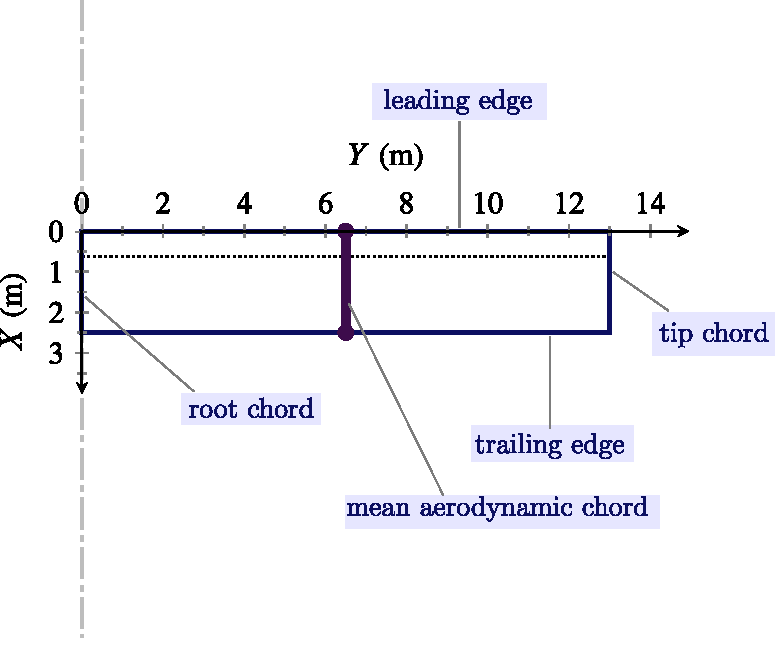
\includegraphics[width=0.78\textwidth]{Chapter_2/geometric_characteristics_of_a_straight_wing/wing_planform_basic_0_drawing.pdf}%
  \caption{\finalhyphendemerits=1000
          Planform of the wing assigned in the example~\ref{example:Geometric:Characteristics:Of:A:Straight:Wing}.}
  \label{fig:Wing:Planform:Basic:Drawing:AA}%
\end{figure}
%
%-------------------------------------------------
%
\def\mySpanWingMT{26.000000}
\def\myChordRootWingMT{2.500000}
\def\myChordTipWingMT{2.500000}
\def\myTaperRatioWing{1.000000}
\def\myAreaWingMTsquared{65.000000}
\def\myMACWingMT{2.500000}
\def\myYMACWingMT{6.500000}
\def\myXLEMACWingMT{0.000000}
\def\myLambdaCQuarter{0.000000}
\def\myLambdaLEDeg{0.000000}
\def\myLambdaLERad{0.000000}
\def\myAspectRatioWing{10.400000}

%


\begin{myExampleX}{Geometric characteristics of a straight wing}{\ding{46}}% \ \Keyboard\ %
\label{example:Geometric:Characteristics:Of:A:Straight:Wing}
%
\noindent
Let's consider a wing with a finite wingspan equal to $b=\SI[round-precision=1]{\mySpanWingMT}{\metre}$, with straight leading and trailing edges and null sweep angle, that is $\Lambda_{c/4}=\SI[round-precision=0]{\myLambdaCQuarter}{\degree}$.
In addition, the wing sections at the various stations $Y$ along the wingspan have constant chord equal to $\SI[round-precision=2]{\myChordRootWingMT}{\metre}$
and they all have the same profile, i.e. the aerodynamic characteristics of the section are constant. We want to calculate the following quantities:
\noindent
\adjustbox{center=\textwidth}{%
$S$\,, $\AR$\,, $\bar{c}$\,, $X_{\mathrm{le},\bar{c}}$\,, $Y_{\bar{c}}$
}% \,, $Y_{\bar{c}}$
\medskip
\noindent
Not being tapered, the wing has a root chord:
$c_\mathrm{r}=\SI[round-precision=2]{\myChordRootWingMT}{\metre}$,
a tip chord $c_\mathrm{t}=\SI[round-precision=2]{\myChordTipWingMT}{\metre}$
and a taper ratio $\lambda=\SI[round-precision=0]{\myTaperRatioWing}{}$.
The leading edge sweep angle is:
 $\Lambda_\mathrm{le}=\SI[round-precision=0]{\myLambdaCQuarter}{\degree}$.
\noindent
The wing surface is calculated as follows:
\[
\begin{split}
S & {}= \frac{b}{2} \, c_\mathrm{r} \, \big( 1 + \lambda \big) = b\,c_\mathrm{r}\\
  & {}=
    \num{0.5} \cdot \SI[round-precision=1]{\mySpanWingMT}{\metre}
      \cdot \SI[round-precision=2]{\myChordRootWingMT}{\metre}
      \cdot \big( 1 + \SI[round-precision=0]{\myTaperRatioWing}{} \big) 
    = { \SI[round-precision=1]{\myAreaWingMTsquared}{\metre^2} }
\end{split}
\]
In this case it is simply the area of a rectangle.
\noindent
The elongation is therefore:
\[
\AR 
  = \frac{b^2}{S}
  = \frac{\big(\SI[round-precision=1]{\mySpanWingMT}{\metre}\big)^2}{\SI[round-precision=1]{\myAreaWingMTsquared}{\metre^2}}
  ={ \num[round-precision=2]{\myAspectRatioWing} }
\]
This value is greater than $\num[round-precision=0]{10}$,so that allows us to say that we are in presence of a wing with an high aspect ratio.
\noindent
The mean aerodynamic chord is given by:
\[
\begin{split}
\bar{c} & {}= \frac{2}{3} \, c_\mathrm{r} \, \frac{1+\lambda + \lambda^2}{1+\lambda} \\
  & {}=
    \num{0.667} \cdot \SI[round-precision=2]{\myChordRootWingMT}{\metre}
      \cdot 
        \frac{
          1 + \SI[round-precision=0]{\myTaperRatioWing}{} + \SI[round-precision=0]{\myTaperRatioWing}{}^2
        }{
          1 + \SI[round-precision=0]{\myTaperRatioWing}{}
        }
    = \SI[round-precision=2]{\myMACWingMT}{\metre} 
\end{split}
\]
Note that for wings like this, the value of $\bar{c} $ is nothing other than that of the chord of any wing section.
\noindent
The longitudinal distance of the leading edge of the mean aerodynamic chord from the leading edge of the root chord is given by:
\[
\begin{split}
X_{\mathrm{le},\bar{c}} 
  & {}=
    \frac{b}{6} \, \frac{1+2\lambda}{1+\lambda} \tan\Lambda_\mathrm{le} \\[3pt]
  & {}=
    \frac{\SI[round-precision=1]{\mySpanWingMT}{\metre}}{6}
      \cdot 
      \frac{
        1 + 2\cdot\SI[round-precision=0]{\myTaperRatioWing}{}
      }{
        1 + \SI[round-precision=0]{\myTaperRatioWing}{}
      }
      \cdot \tan \big( \SI[round-precision=0]{\myLambdaLERad}{\radian} \big)
    = { \SI[round-precision=0]{\myXLEMACWingMT}{\metre} }% \myXLEMACWingMT
\end{split}
\]
The null value confirms that the mean aerodynamic chord, projected on the center plane of the wing, overlaps the root chord.
\noindent
For the assigned wing, all the stations $Y$ along the wingspan have a chord equal to $\bar{c}$. Formally, the station $Y_{\bar{c}}$ corresponding to the mean aerodynamic chord is calculated as follows:
\[
\begin{split}
Y_{\bar{c}} 
  & {}=
    \frac{b}{6} \, \frac{1+2\lambda}{1+\lambda} = \\[3pt]
  & {}=
    \frac{\SI[round-precision=1]{\mySpanWingMT}{\metre}}{6}
      \cdot 
      \frac{
        1 + 2\cdot\SI[round-precision=2]{\myTaperRatioWing}{}
      }{
        1 + \SI[round-precision=2]{\myTaperRatioWing}{}
      }
    = { \SI[round-precision=2]{\myYMACWingMT}{\metre} }
    = \frac{b}{2} \, \frac{1}{2}
\end{split}
\]
The value obtained corresponds to the station along the wingspan halfway between the root chord and the tip chord. We will see later that for this type of straight wing with constant section, when twisting geometric $\epsilon_\mathrm{g}(Y)$ is identically null,the basic aerodynamic characteristics of the section profile are transferred to the finished wing. For example, the zero lift angle $\alpha_{0L}$ coincides with  zero lift angle $\alpha_{0\ell}$ of the profile; just as $C_L \big|_{\alpha = 0} $ coincides with the profile $C_{\ell 0}$. The gradient \smash{$C_{L_\mathlarger{\alpha}}$} relative to the wing must instead be corrected respect to the value of \smash{$C_{\ell_\mathlarger{\alpha}}$} relative to the profile for the finite elongation effect.
\end{myExampleX}
\end{document}
